\documentclass[a4paper, 14pt]{extarticle}

% file's preambule

% Если вы работаете не в XeLaTeX, то сами разбирайтесь =)

% connect packages
%%%%%%%%%%%%%%%%%%%%%%%%%%%%%%%%%%%%%%%%%%%%%%%%%%%%%%%%%%%%%%%%%%%%%%
%\usepackage[T2A]{fontenc}                   %!? закрепляет внутреннюю кодировку LaTeX
%\usepackage[utf8]{inputenc}                 %!  закрепляет кодировку utf8
\usepackage{fontspec}                        % Шрифты
\usepackage{indentfirst}                    %   добавить indent перед первым параграфом
\setlength{\parindent}{1.27cm}
\usepackage{polyglossia}                     % Русский язык
\setdefaultlanguage{russian}
\setmainfont[Ligatures=TeX]{Times New Roman}
\newfontfamily\cyrillicfont{Times New Roman}[Script=Cyrillic]
%\usepackage[english,russian]{babel}         %!  подключает русский и английский
\usepackage{amsmath}                        %!  |
\usepackage{amssymb,textcomp, esvect,esint} %!  |важно для формул 
\usepackage{geometry}                       %!  отступ от граней
\geometry{verbose,a4paper,tmargin=2cm,bmargin=2cm,lmargin=3cm,rmargin=1cm}
\usepackage{amsfonts}                       %!  математические шрифты
\usepackage{amsthm}                         %!  newtheorem и их сквозная нумерация
\usepackage{graphicx}                       %?  графическое изменение текста
\usepackage{soulutf8}% Поддержка переносоустойчивых подчёркиваний и зачёркиваний
\usepackage{enumitem}                       %!  задание макета перечня.
%\usepackage[unicode, pdftex]{hyperref}      %!  оглавление для панели навигации по PDF-документу + гиперссылки
\usepackage{setspace}                       % Межстроковые интервалы
\onehalfspacing
\usepackage{booktabs}                       %!  добавляет книжные линии в таблицы
%\usepackage{hypcap}                         %?  адресация на картинку, а не на подпись к ней
\usepackage{abraces}                        %?  фигурные скобки сверху или снизу текста
\usepackage{caption}                        %-  позволяет корректировать caption 
\DeclareCaptionLabelSeparator{dash}{ - }
\captionsetup[table]{labelformat=simple, labelsep=dash, justification=raggedleft,
singlelinecheck=off}
\captionsetup[figure]{labelformat=simple, labelsep=dash}
\usepackage{multirow}                       %   объединение ячеек в таблицах
\usepackage{longtable}
\usepackage{pifont}                         %!  нужен для крестика
\usepackage{cancel}                         %!  аутентичное перечеркивание текста
\usepackage{ulem}                           %!  перечеркивание текста
\usepackage{tikz}                           %!  высокоуровневые рисунки (кружочек)
\usepackage{titling}                        %-  автоматическое заглавие 
\usepackage{titlesec}  % нормальные заголовки секций
\titleformat{\section}
{\normalfont\large\bfseries\filcenter}{}{1em}{}
\titleformat{\subsection}
  {\normalfont\normalsize\bfseries}{\thesubsection.}{5pt}{}
\titleformat{\subsubsection}
  {\normalfont\normalsize\bfseries}{\thesubsubsection.}{5pt}{}
\titleformat{\paragraph}
  {\normalfont\normalsize\bfseries}{\theparagraph}{5pt}{}

\usepackage{ragged2e} % Для выравнивания текста по ширине
\justifying

%\renewcommand{\thesubsubsection}{\alph{subsubsection}}
\usepackage{blindtext}                      %-  слепой текст
\usepackage{fancyhdr}                       %   добавить верхний и нижний колонтитул
\usepackage{mathptmx}

\usepackage{import}                         %|
\usepackage{xifthen}                        %|
\usepackage{pdfpages}                       %|
%\usepackage{transparent}                    %| вставка ink figures
\usepackage{rotating}
\usepackage{array} % Картиночки в таблицы
%%%%%%%% Алгоритмы
\usepackage{float}
\usepackage{algorithm}
\usepackage{algpseudocode}
%%%%%%%%%%%%%%%

\usepackage{listings} % Для языков программирования 
\usepackage{xcolor}
\lstset {
    language=C++,
    backgroundcolor=\color{black!5}, % set backgroundcolor
    basicstyle=\footnotesize,% basic font setting
}

\usepackage{lmodern}

\colorlet{comment}{green!50!black}
\colorlet{cppcomment}{teal}
\colorlet{symb}{blue!50!black}
\colorlet{number}{violet}

\newcommand*{\textcolorsymb}{\textcolor{symb}}

\definecolor{backcolour}{rgb}{0.95,0.95,0.92}
\definecolor{black_red}{rgb}{0.54, 0, 0}

\lstdefinestyle{cpp}{%
  language=C++,
  columns=flexible,
  basewidth=.5em,  
  tabsize=2,
  basicstyle=\footnotesize,
  backgroundcolor=\color{backcolour},
  showspaces=false,
  showstringspaces=false,
  commentstyle={\itshape\color{comment}\let\textcolorsymb\relax},
  keywordstyle=\bfseries\color{black_red},
  morecomment={[l][\itshape\color{cppcomment}\let\textcolorsymb\relax]//},
  literate=%
    {\{}{\textcolorsymb{\{}}1
    {\}}{\textcolorsymb{\}}}1
    {(}{\textcolorsymb{(}}1
    {)}{\textcolorsymb{)}}1
    {;}{\textcolorsymb{;}}1
    {=}{\textcolorsymb{=}}1
    {<}{\textcolorsymb{<}}1
    {>}{\textcolorsymb{>}}1
    {!}{\textcolorsymb{!}}1
    {\&}{\textcolorsymb{\&}}1 
    {|}{\textcolorsymb{|}}1
    {?}{\textcolorsymb{?}}1
    {:}{\textcolorsymb{:}}1
    {+}{\textcolorsymb{+}}1
    {-}{\textcolorsymb{-}}1
    {,}{\textcolorsymb{,}}1
    {\%}{\textcolorsymb{\%}}1
    {\^}{\textcolorsymb{\textasciicircum}}1
    {~}{\textcolorsymb{\textasciitilde}}1
    %% {/}{\textcolorsymb{/}}1
    %% {*}{\textcolorsymb{*}}1
    % 2 (optionally)
    {==}{\textcolorsymb{==}}2
    {>=}{\textcolorsymb{=>}}2
    {<=}{\textcolorsymb{<=}}2
    {!=}{\textcolorsymb{!=}}2
    {+=}{\textcolorsymb{+=}}2
    {-=}{\textcolorsymb{-=}}2
    {*=}{\textcolorsymb{*=}}2
    {/=}{\textcolorsymb{/=}}2
    {\%=}{\textcolorsymb{\%=}}2
    {\&\&}{\textcolorsymb{\&\&}}2
    {||}{\textcolorsymb{||}}2
    {++}{\textcolorsymb{++}}2
    {--}{\textcolorsymb{--}}2
    {>>}{\textcolorsymb{>\kern0pt>}}2
    {<<}{\textcolorsymb{<\kern0pt<}}2
    {::}{\textcolorsymb{::}}2
    % 3 (optionally)
    {>>=}{\textcolorsymb{>\kern0pt>=}}3
    {<<=}{\textcolorsymb{<\kern0pt<=}}3
    % Remove byte order mark
    {^^ef^^bb^^bf}{}0
}
\lstnewenvironment{cpp}{\lstset{style=cpp}}{}
\lstset{style=cpp}
  


%%%%%%%%%%%%%%%%%%%%%%%%%%%%%%%%%%%%%%%%%%%%%%%%%%%%%%%%%%%%%%%%%%%%%%


%%%%%%%%%%%%%%%%%% ВСТАВКА РИСУНКО ИЗ INKSCAPE %%%%%%%%%%%%%%%%%%%%%%%
\newcommand{\incfig}[1]{%
    \def\svgwidth{\columnwidth}
    \import{./figures/}{#1.pdf_tex}
}

%%%%%%%%%%%%%%%%%%%%%%%%%%%%%%%%%%%%%%%%%%%%%%%%%%%%%%%%%%%%%%%%%%%%%%


\newenvironment{itemize*}
{
    \begin{itemize}
        \setlength{\itemsep}{1pt}
        \setlength{\parskip}{1pt}}
    {\end{itemize}
}

\newenvironment{enumerate*}
{
    \begin{enumerate}
        \setlength{\itemsep}{1pt}
        \setlength{\parskip}{1pt}}
    {\end{enumerate}
}

%%%%%%%%%%%%%%%%%%%%%%%%%%%%%%%%%%%%%%%%%%%%%%%%%%%%%%%%%%%%%%%%%%%%%%


\begin{document}
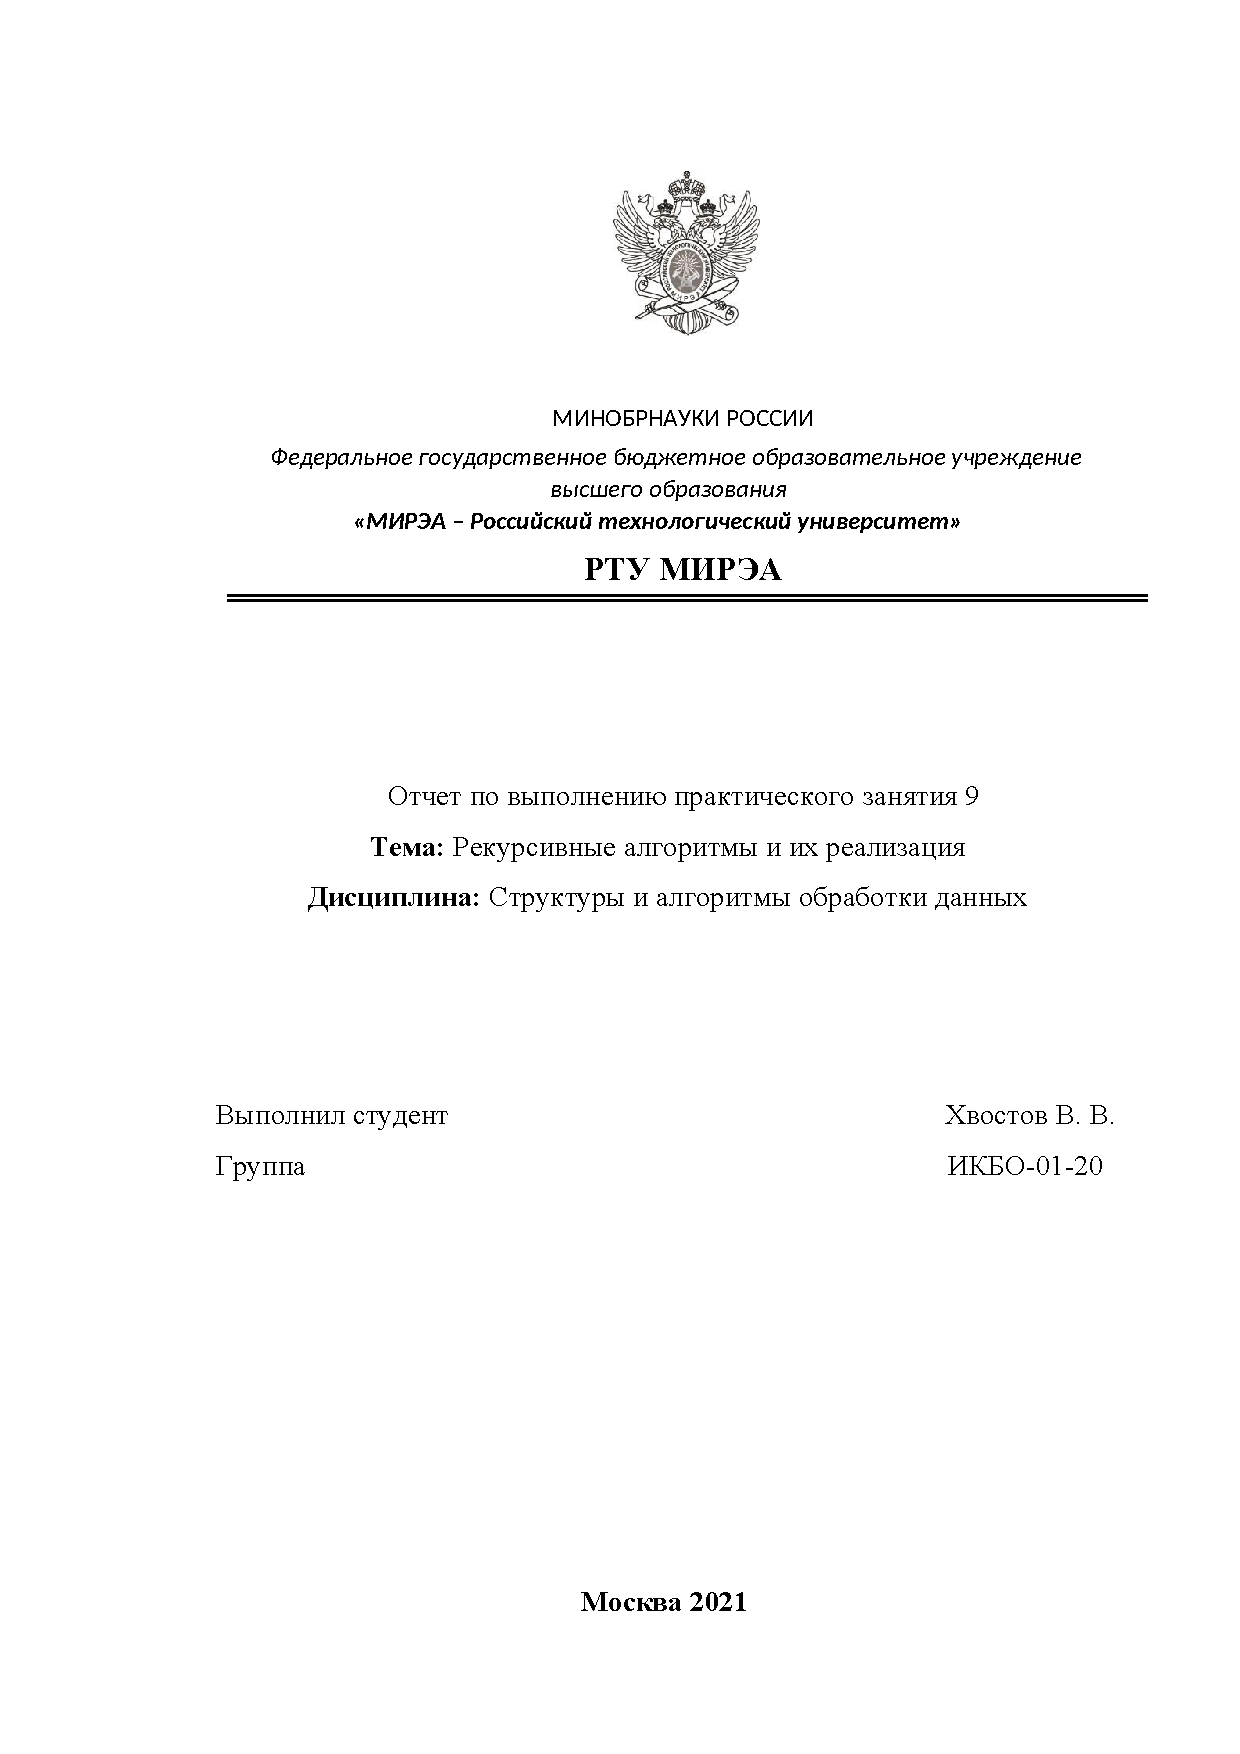
\includepdf{titul_ninth}
\newpage
\tableofcontents
\newpage
\section{Ответы на вопросы}
\paragraph{Рекурсивная функция}
Рекурсивная функция - числовая функция числового аргумента,
которая в своём определении содержит себя же (математическое определение).

Рекурсивная функция -это функция, которая вызывает саму себя (в языках программирования).
\paragraph{Шаг рекурсии}
Шаг рекурсии - это условие продолжения рекуррентного вызова.
\paragraph{Глубина рекурсии}
Глубина рекурсии - это количество одновременно выполняемых процедур.
\paragraph{Условие завершения рекурсии}
Условие завершения рекурсии - это условие, которое, при его выполнении,
остановит вызов рекурсивной функции самой себя.
\paragraph{Линейная рекурсия}
Линейная рекурсия - вид рекурсии, при которой рекурсивные вызовы
на любом рекурсивном срезе, инициируют
не более одного последующего рекурсивного вызова.
\paragraph{Каскадная рекурсия}
Каскадная рекурсия - рекурсия, не являющаяся линейной.
При каскадной рекурсии, рекурсивные обращения, как правило,
приводят к необходимости многократно решать одни и те же подзадачи.
\paragraph{Прямая рекурсия}
Прямая  рекурсия  вызывает  алгоритм (функцию, процедуру)
P из текста самого алгоритма P.
\paragraph{Косвенная рекурсия}
Косвенная рекурсия - циклическая последовательность вызовов нескольких алгоритмов
$P_1, P_2, \ldots, P_n$ (функций, процедур) друг друга:
$P_1$ вызывает $P_2$, $P_2$ вызывает $P_3$, $\ldots$, $P_n$ вызывает $P_1$ ($n > 1$).
\paragraph{Организация стека рекурсивных вызовов}
Стек рекурсии - область памяти, в которую заносятся значения
всех локальных переменных алгоритма (программы) в момент рекурсивного обращения.
Каждое такое обращение формирует один слой данных стека.
При завершении вычислений по конкретному обращению $a$ из стека считывается
соответствующий ему слой данных, и локальные переменные восстанавливаются,
снова принимая значения, которые они имели в момент обращения $a$.
\newpage
\section{Главное задание}
\textit{Вариант 10}
\subsection{Задача 1}
\subsubsection{Условие задачи}
Вычислить значение цифрового корня для некоторого целого числа N.
\subsubsection{Постановка задачи}
Реализовать функцию вычисления произвольного корня для некоторого целого числа N.
\subsubsection{Описание алгоритма – рекуррентная зависимость}
Для реализации данной функции воспользуемся методом Ньютона из математического
анализа, который позволяет найти приблизительное значение функции в конкретной
точке (в нашем случае $f(x)=x^{\frac{1}{n}} $, где $n\in \mathbf{N}$).
Рекуррентным соотношение в данном случае является формула
\[
  x_{k+1}=\frac{1}{n}\left ((n-1)x_k+\frac{N}{x_k^{n-1}}\right )
.\] где $x_k$ - значение $x$ на $k$ шаге рекурсии. Чем больше количество
вызовов рекурсии, тем точнее наш результат. Но т.к. компьютер ограничен в точности,
то мы зададим условие выхода из рекурсии такое, чтобы разница между $x_n$ и
$x_{n+1}$ была меньше определенной константы $h$, определенной ниже.
\subsubsection{Коды используемых функций}
\lstinputlisting[lastline=13]{code/recur_funs.cpp}
\subsubsection{Ответы на задания по задаче 1}
\paragraph{Итерационный алгоритм решения задачи}
Для решения данной задачи можно использовать алгоритм, который сравнивает разность
текущего и предыдущего значения x с некоторой погрешностью в цикле и каждый
раз считает новое значение корня n-ой степени, сохраняя предыдущее для следующей
итерации.
\paragraph{Реализация в виде функции для итерационного алгоритма}
\lstinputlisting[firstline=15, lastline=26]{code/recur_funs.cpp}
\paragraph{Теоретическая сложность алгоритма}
Теоретическая сложность алгоритма равна $\Theta(d^p\lg d)$ т.к.
каждый раз в цикле точность увеличивается примерное в $p$ раз, а также
$\Theta(d^p)$ - сложность выполнения возведения в степень(где $p$ - степень корня,
$d$ - необходимая точность результата т.е. количество цифр после запятой).
\paragraph{Рекуррентная зависимость}
Рекуррентная зависимость в данной задаче - значение корня k-ой степени,
вычисленное на предыдущем шаге.
\paragraph{Реализация в виде функции для рекуррентного алгоритма}
\lstinputlisting[lastline=13]{code/recur_funs.cpp}
\paragraph{Глубина рекурсии}
Условием выхода из рекурсии является вычисление корня с необходимой точностью т.е.
из теоретической сложности получаем, что глубина алгоритма = $\lg d$ (т.к.
на каждом уровне происходит умножением со сложностью $\Theta(d^p)$).
\paragraph{Определение сложности рекурсивного алгоритма}
Определим сложность рекурсивного алгоритма с помощью метода постановки
и дерева рекурсии. Пусть у нас на вход подается какое-то число с количеством
знаков в результате d. Построим для него дерево
(рис. \ref{fig:tree1}).
\begin{figure}[htpb]
  \centering
  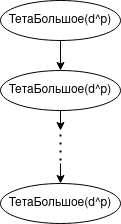
\includegraphics[width=0.2\textwidth]{pictures/tree1.png}
  \caption{Дерево рекурсии для задания 1}
  \label{fig:tree1}
\end{figure}
Суммируя все узлы дерева, получаем сложность $\Theta(d^p\lg d)$ (т.к. глубина дерева =  $ \lg d$).
\newpage
\paragraph{Пример схемы рекурсивных вызовов}
\begin{figure}[htpb]
  \centering
  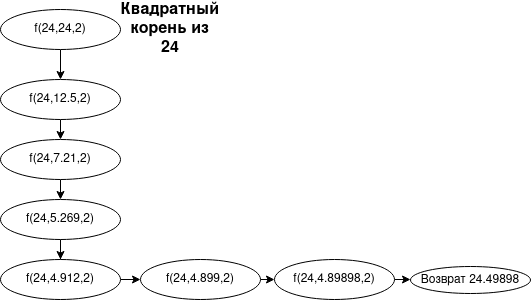
\includegraphics[width=0.6\textwidth]{pictures/tree1_ex.png}
  \caption{Пример рекурсии задания 1}
  \label{fig:tree1_ex}
\end{figure}
\subsubsection{Код программы}
\lstinputlisting[firstline=28]{code/recur_funs.cpp}
\subsubsection{Результаты тестирования}
\begin{table}[htpb]
  \centering
  \caption{Тестирование задачи 1}
  \label{tab:task1_test}
  \begin{tabular}{|c|c|c|c|}
    \hline
    \parbox[c]{15mm}{\centering Номер \\ теста} & Входные данные &
    \parbox[m]{3cm}{\centering Ожидаемый \\ результат} &
    \parbox[m]{3cm}{\centering Результат \\ выполнения программы}
    \\ \hline
    1 & \parbox[c]{5cm}{\centering Число: 24,\\Степень: 2}
      & \parbox[m]{3cm}{\centering 4.89898} & \raisebox{-.5\height}
      {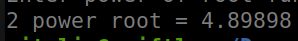
\includegraphics[width=65mm]{pictures/task1_test1.png}} \\ \hline
    2 & \parbox[c]{5cm}{\centering Число: 1324,\\Степень: 3}
      & \parbox[m]{3cm}{\centering 10.9807} & \raisebox{-.5\height}
      {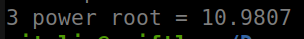
\includegraphics[width=65mm]{pictures/task1_test2.png}} \\ \hline
    3 & \parbox[c]{5cm}{\centering Число: 256,\\Порядок: 4}
      & \parbox[m]{3cm}{\centering 4} & \raisebox{-.5\height}
      {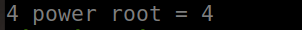
\includegraphics[width=65mm]{pictures/task1_test3.png}} \\ \hline
  \end{tabular}
\end{table}
\subsection{Задача 2}
\subsubsection{Условие задачи}
Найти в двунаправленном списке количество четных элементов.
\subsubsection{Постановка задачи}
Реализовать функцию поиска количества четных элементов в двунаправленном списке.
\subsubsection{Описание алгоритма – рекуррентная зависимость}
Для решения задачи с помощи рекурсии каждый раз мы будем рассматривать элемент
в списке, на который наш указатель хранит адрес, проверять является ли он четным,
и затем вызывать рекурсивно эту же функцию, но для следующего элемента.
Алгоритм заканчивает свою работу при достижении конца списка.
\subsubsection{Коды используемых функций}
\lstinputlisting[lastline=16]{code/second_rec.cpp}
\subsubsection{Ответы на вопросы задания 2}
\paragraph{Глубина рекурсии}
Глубина рекурсии равна $n$ т.е. размеру списка т.к. нам требуется пройти
по всему списку для подсчета количества четных элементов.
\paragraph{Теоретическая сложность алгоритма}
Теоретическая сложность алгоритма равна $\Theta(n)$ т.к. мы полностью
проходим список 1 раз.
\subsubsection{Код программы}
\lstinputlisting[firstline=16]{code/second_rec.cpp}
\newpage
\subsubsection{Результаты тестирования}
\begin{table}[htpb]
  \centering
  \caption{Тестирование задачи 2}
  \label{tab:task2_test}
  \begin{tabular}{|c|c|c|c|}
    \hline
    \parbox[c]{15mm}{\centering Номер \\ теста} & Входные данные &
    \parbox[m]{3cm}{\centering Ожидаемый \\ результат} &
    \parbox[m]{3cm}{\centering Результат \\ выполнения программы}
    \\ \hline
    1 & \parbox[c]{5cm}{\centering Список: 7 10 7 7 5 6 1 4 6 4}
      & \parbox[m]{3cm}{\centering 5} & \raisebox{-.5\height}
      {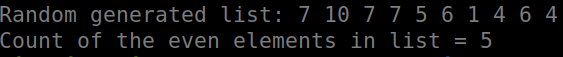
\includegraphics[width=65mm,height=13mm]{pictures/task2_test1.png}} \\ \hline
    2 & \parbox[c]{5cm}{\centering Список: 1 1 5 7 9 1 2 1 10 8}
      & \parbox[m]{3cm}{\centering 3} & \raisebox{-.5\height}
      {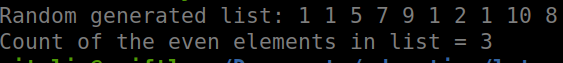
\includegraphics[width=65mm,height=13mm]{pictures/task2_test2.png}} \\ \hline
    3 & \parbox[c]{5cm}{\centering Список: 6 7 4 2 9 7 3 6 2 4}
      & \parbox[m]{3cm}{\centering 6} & \raisebox{-.5\height}
      {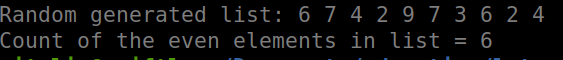
\includegraphics[width=65mm, height=13mm]{pictures/task2_test3.png}} \\ \hline
  \end{tabular}
\end{table}
\newpage
\section*{Выводы}
\addcontentsline{toc}{section}{Выводы}
В ходе выполнения работы были получены практические навыки
по разработке рекурсивных алгоритмов. В соответствии с
персональным вариантом, были созданы и проанализированы следующие
рекурсивные (и итеративные) алгоритмы: функция подсчета корня n-ой
степени, подсчет количества четных чисел в двунаправленном списке.
Каждая рекурсивная функция прошла тестирование успешно, что подтверждает правильную
работу алгоритмов.
\section*{Список информационных источников}
\addcontentsline{toc}{section}{Список информационных источников}
\begin{enumerate}[leftmargin=*]
  \item Thomas H. Cormen, Clifford Stein и другие: Introduction to Algorithms, 3rd Edition.
    Сентябрь 2009. The MIT Press.
  \item Олег Смирнов: Анализ рекуррентных соотношений . Октябрь 2011.
    \\ https://nord.org.ua/static/course/algo\_2011/lecture2.pdf.
  \item Nth root~//~Wikipedia \\~
    [Электронный ресурс]. URL:
    \\ https://en.wikipedia.org/wiki/Nth\_root
    (Дата обращения: 07.05.2021)
   \item Курс Algorithms, part 2 // Coursera [Электронный ресурс]. URL:
     \\ https://www.coursera.org/learn/algorithms-part2
     (Дата обращения: 07.05.2021)
\end{enumerate}
\end{document}
